\documentclass[a4paper, 12pt]{article}

\usepackage[utf8]{inputenc}
\usepackage[T1]{fontenc}
\usepackage[english, francais]{babel}
\usepackage{graphicx}
\usepackage{listings}
\usepackage{color}
\usepackage{enumerate}

\definecolor{codegreen}{rgb}{0,0.6,0}
\definecolor{codegray}{rgb}{0.5,0.5,0.5}
\definecolor{codepurple}{rgb}{0.58,0,0.82}
\definecolor{backcolour}{rgb}{0.95,0.95,0.92}

\newcommand{\Hrule}{\rule{\linewidth}{0.5mm}}

\lstdefinestyle{mystyle}{
    backgroundcolor=\color{backcolour},   
    commentstyle=\color{codegreen},
    keywordstyle=\color{magenta},
    numberstyle=\tiny\color{codegray},
    stringstyle=\color{codepurple},
    basicstyle=\footnotesize,
    breakatwhitespace=false,         
    breaklines=true,                 
    captionpos=b,                    
    keepspaces=true,                 
    numbers=left,                    
    numbersep=5pt,                  
    showspaces=false,                
    showstringspaces=false,
    showtabs=false,                  
    tabsize=2
}

\lstset{language=C++,
    basicstyle=\small,
    keywordstyle=\color{blue}\small,
    stringstyle=\color{red}\small,
    commentstyle=\color{green}\small,
    morecomment=[l][\color{magenta}]{\#},
    tabsize=2
}

\title{Le Vouitris}
\date{13 mars 2019}
\author{Cynthia MAILLARD \and Alexandre DILLON \and Félix ROYER}

\begin{document}

\begin{titlepage}
        
    \begin{figure}
       \begin{minipage}[c]{.46\linewidth}
            
\includegraphics[scale=0.5]{img/logU.png} 
       \end{minipage} \hfill
       \begin{minipage}[c]{.46\linewidth}
              
\includegraphics[scale=0.08]{img/logF.jpg} 
       \end{minipage}
    \end{figure}

    \begin{sffamily}
    \begin{center}

    \textsc{Université de Franche-Comté}\\[0.2cm]
     L3 CMI Informatique\\[0.5cm]

    \textsc{Projet intégrateur}\\[0.5cm]

    \Hrule \\[0.2mm]

    { \huge \bfseries Tétris en réseau - Le Vouitris\\[0.8mm]}

    \Hrule\\[1cm]

    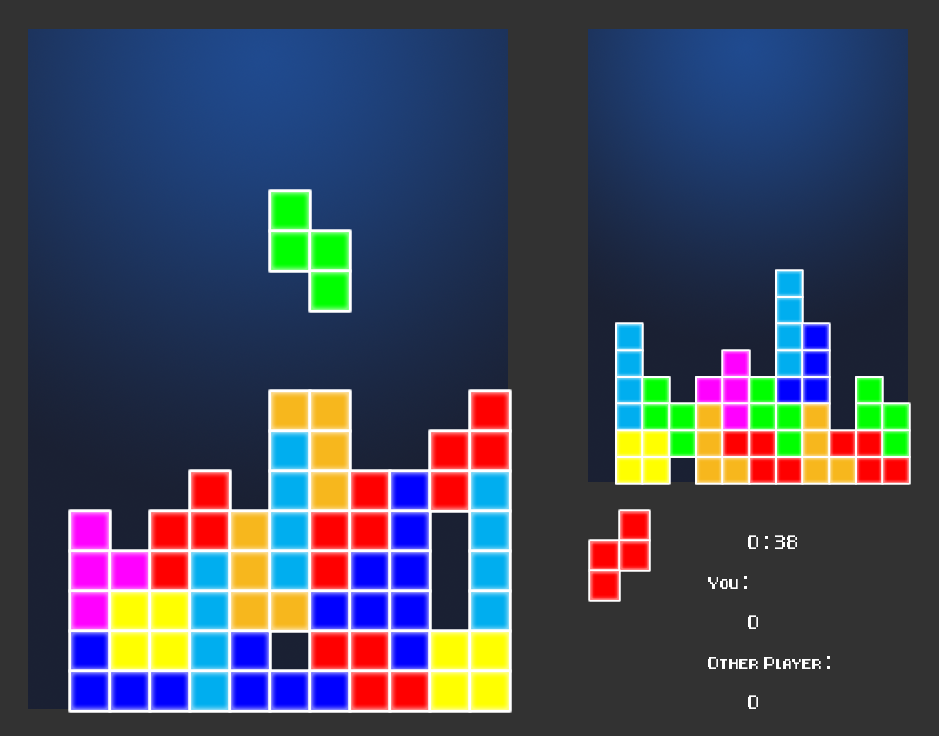
\includegraphics[scale=0.30]{img/vouitris.png} 

    \vspace{1cm}

    \Large{Cynthia MAILLARD, Alexandre DILLON, Félix ROYER} \\

    \vspace{0.25cm}

    \Large{\underline{Tuteur de projet} : Julien BERNARD}
    
    \vspace{0.5cm}

    {\large Année universitaire 2018-2019}

    \end{center}
    \end{sffamily}
    \thispagestyle{empty}% Ne numérote pas la page


\end{titlepage}

\newpage

\tableofcontents

\newpage

\section*{Remerciements}

Nous tenons à remercier Monsieur Julien Bernard, notre encadrant pour ce projet, pour le soutien qu'il nous apporté tout au long du développement ainsi que l'aide pour la préparation de la soutenance et de ce rapport.

\newpage
	
\section*{Introduction}
	La réalisation de ce projet s'inscrit dans le cadre du projet intégrateur de notre troisième année de licence informatique à l'Université de Besançon. Pour ce projet, nous avons réalisé le sujet proposé par Julien Bernard, enseignant-chercheur en informatique à l'Université de Franche-Comté : un tétris multijoueur en réseau.

	\bigskip

	Le but est de développer notre version du célèbre jeu de puzzle, en faisant s'affronter deux joueurs l'un contre l'autre. Nous devons donc concevoir des interfaces graphiques pour les joueurs et créer un réseau pour permettre aux joueurs de jouer ensemble.

	\bigskip

	Le développement devait être fait en C++, avec la bibliothèque Boost.asio pour la communication réseau et les parties graphiques devait être réalisées en utilisant la bibliothèque Gamedev Framework, bibliothèque conçue pour le développement de jeux vidéo, développée par Julien Bernard.
	Le développement s'étendait d'octobre 2018 à mars 2019.

	\bigskip
	Nous étions intéressés par ce projet car nous voulions améliorer nos connaissances dans le language C++. De plus la simplicité de la conception d'un Tétris nous permettait d'approfondir certains domaines spécifiques liés au développement, tel que approfondir la programmation distribuée et la sérialisation nous motivait pour ce projet.

	\bigskip
	Ce rapport a pour but de rendre compte du travail que nous avons réalisé au cours du projet.

	\newpage

\section{Adaptation du jeu d'origine}
	\subsection{Tétris originel}		


		Tetris est un jeu vidéo de puzzle conçu par Alekseï Pajitnov en 1984. Tetris est principalement composé d'une zone de jeu où des pièces de formes différentes, appelées « tétrominos » --- dont les différentes formes sont représentée sur la figure \ref{fig:tetros} ---, descendent du haut de l'écran. 
		
		\begin{figure}[tb]
			\centering
			\includegraphics[scale=0.2]{img/tetros.png}
			\caption{Les différentes formes de tétromino}
			\label{fig:tetros}
		\end{figure}

		Durant la chute des tetrominos, le joueur peut déplacer les pièces latéralement, leur faire effectuer une rotation sur elles-mêmes et dans certaines versions, accélérer la vitesse de chute jusqu'à ce qu'elles se pose sur le bas de la zone de jeu ou sur une autre pièce. 
		
		Le but pour le joueur est de réaliser le plus de lignes possibles. Une fois une ligne complétée, elle disparaît, et les blocs placés au-dessus chutent d'un rang. 
		Lorsque le joueur accumule les pièce et remplie la zone de jeu jusqu’en haut, ce qui empêche l'arrivée de tétriminos supplémentaires, la partie se termine. Le joueur obtient un score, qui dépend essentiellement du nombre de lignes réalisées lors de la partie. On ne peut donc jamais gagner à Tetris, le but étant d’améliorer son précédent score.

		Après la version originale du jeu sortie sur l'\textit{Elektronika 60}, le tétris a connu un succès mondial dans les années 1990 grâce à sa version Gameboy, dont on voit une capture d'écran sur la figure \ref{fig:tetris}.

		\begin{figure}[b]
			\centering
			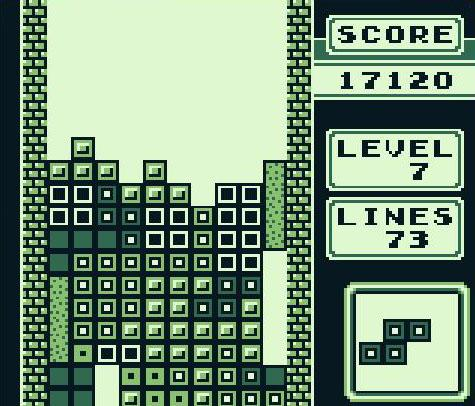
\includegraphics[scale=0.3]{img/Tetris8.jpg}
			\caption{Interface de tétris sur Gameboy}
			\label{fig:tetris}
		\end{figure}
		

		Le jeu a été adapté sur pratiquement toutes les consoles de toutes les générations, soit dans une version strictement identique soit dans une adaptation plus libre ne conservant que certains point du gameplay original. Au début des années 2010, on comptait plus de 65 plate-formes qui possaidait un portage du jeu.

		Tétris s'est imposé comme l'un des plus grands succès de l'histoire du jeu vidéo et l'une de ces icones les plus mondialement connues. Il faut noter également que le jeu a connue des adaptations multijoueurs --- notamment le projet \emph{Tétrinet} à la fin des années 1990 --- et ce encore aujourd'hui, avec par exemple \emph{Tétris 99}, qui est sorti le 13 février 2019 sur Nintendo Switch.

	\subsection{Notre adaptation}
		\subsubsection{Les objectifs du développement}
			Notre adaptation est une version multijoueur du Tétris, où chaque joueur a un jeu qui tourne sur son ordinateur, sur lequel il joue seul avec son clavier. 


			Le but est que chaque joueur possède un client sur son ordinateur, qu'il se connecte en réseau sur un serveur. Le serveur gérerait le déroulement du jeu, servirait d'intermédiaire entre les deux joueurs et centraliserais les données de la partie.
			Les clients n'aurait accès qu'aux données minimum requises pour afficher le jeu et communiquer leurs actions au serveur. 


			Nous devions donc développer un serveur capable de gérer le jeu et de communiquer son évolution à des clients et des clients capables d'afficher l'état du jeu tel qu'il est sur le serveur et de lui renvoyer les interactions des joueur.


		\subsubsection{Les contraintes de développement}
			Cela nous a donné une contrainte à respecter : le serveur fait loi. Les clients ne servent qu'à l'affichage du jeu et à la réception des actions de l'utilisateur, mais ne contrôlent pas le déroulement de la partie.

			De plus nous avons créer un système d'anti-triche afin de contrôler que les action du clients ne soit cohérente avec le déroulement de la partie.

		\subsubsection{Les malus}
			Les joueurs joueront une partie de Tétris classique, chacun de leur coté. Cependant, pour ne pas limiter l'affrontement à un concours de score, nous avons choisi d'ajouter un système de malus.

			Lorsqu'un joueur parvient à détruire des lignes, son adversaires se voit pénalisé plus ou moins sévérement en fonction du nombre de lignes détruites :
			\begin{itemize}
				\item suppression de 2 lignes : le joueur adverse ne peut plus faire de rotation sur ses pièces pendant 10 secondes.
				\item suppression de 3 lignes : la vitesse des chutes des pièce de l’adversaire augmente pendant 10 secondes.
				\item suppression de 4 lignes : certaines case sont enlevé du mur adverse pouvant l’empêcher de compléter certaine lignes.
			\end{itemize}

			Il n'y a pas de malus pour la suppression d'une seule ligne, car les parties était trop déséquillibrées avec.

	\section{Modélisation du jeu}

		\subsection{Architecture réseau}

			Nous avons déjà défini que nous avions besoin d'une architecture client-serveur dans la partie précédente.

			La difficultée etant que les clients et le serveur doivent être capable d'attendre l'arrivé d'un message sur leur socket, tout en exécutant une boucle simultanément --- la fenêtre graphique pour les clients et la boucle de jeu pour le serveur.


			Pour résoudre ce problèmes nous avons séparé la réception des messages dans un thread à part dans les clients et le serveur.

			Ce thread attends la reception d'un message et le place dans une file. Le thread principal récupère ensuite les messages contenu dans cette file et les exploitent, comme on peut le voir sur la figure \ref{fig:rezo}.

			\begin{figure}[bt]
				\centering
				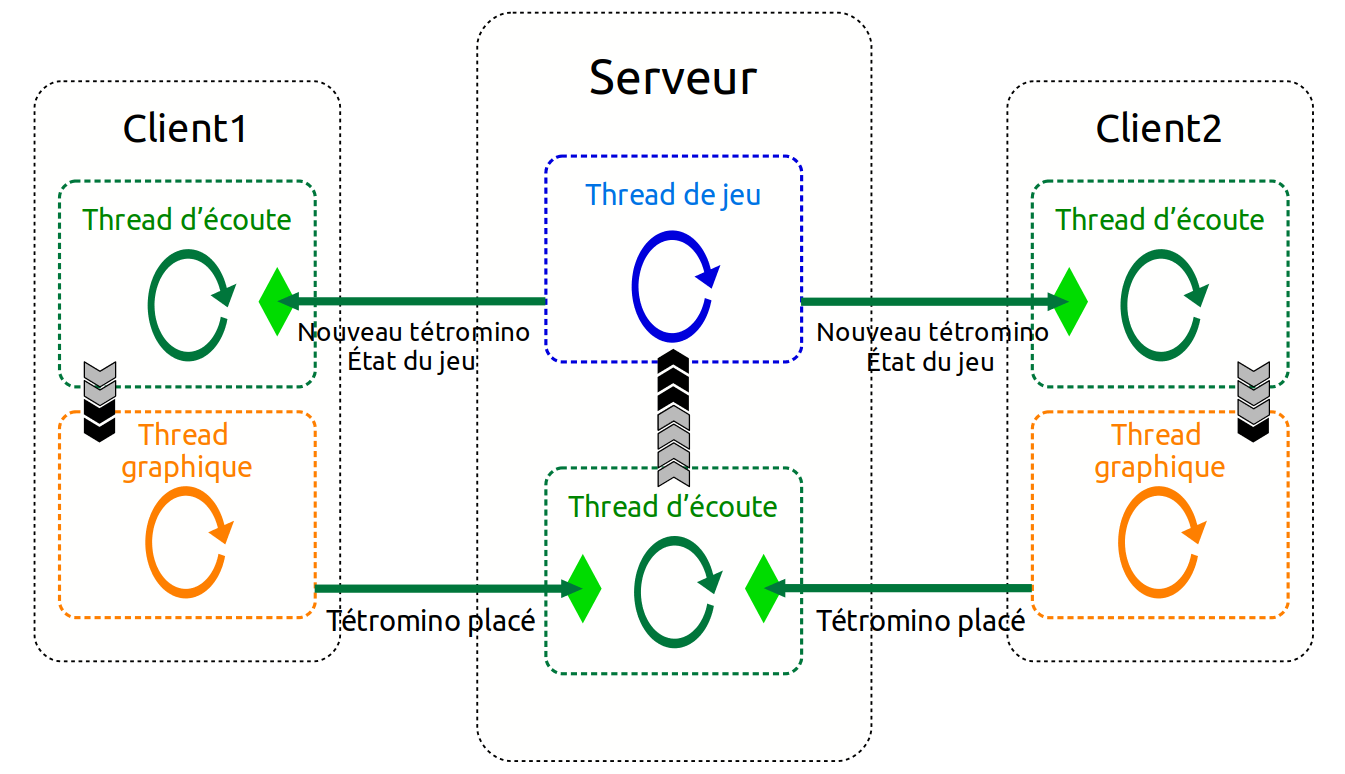
\includegraphics[scale=0.3]{img/archi_reseau.png}
				\caption{Représentation simplifiée de l'architecture réseau entre les clients et le serveur}
				\label{fig:rezo}
			\end{figure}

			Ainsi, les clients et le serveur vont pouvoir s'envoyer des messages sans problèmes, étant donné qu'il y a en permanence une socket qui écoute la réception de message. L'interprétation des messages est faites durant la boucle principale des deux applications, ce qui ne bloque pas leur exécution.

			Le réseau à donc une architecture de réseau temps réel, mais les échanges de messages sont assez peu nombreux, donc notre réseau peut être concidéré comme un réseau temps réel lent.

		\subsection{\'Echanges entre les clients et le serveur}

			Notre protocole d'échange tel que l'avons défini implique que le serveur gère seul la partie, et les clients uniquement l'affichage et les interactions de l'utilisateur.

			Par conséquent, les échanges vont consister en la mise à jour de l'état du jeu de la part du serveur et les actions du joueur de la part du client. 
			La figure \ref{fig:echange} représente une version simplifié des échanges entre les clients et le serveur. Pour des soucis de lisibilité, nous n'avons représenté qu'un seul client.

			\begin{figure}[bt]
				\centering
				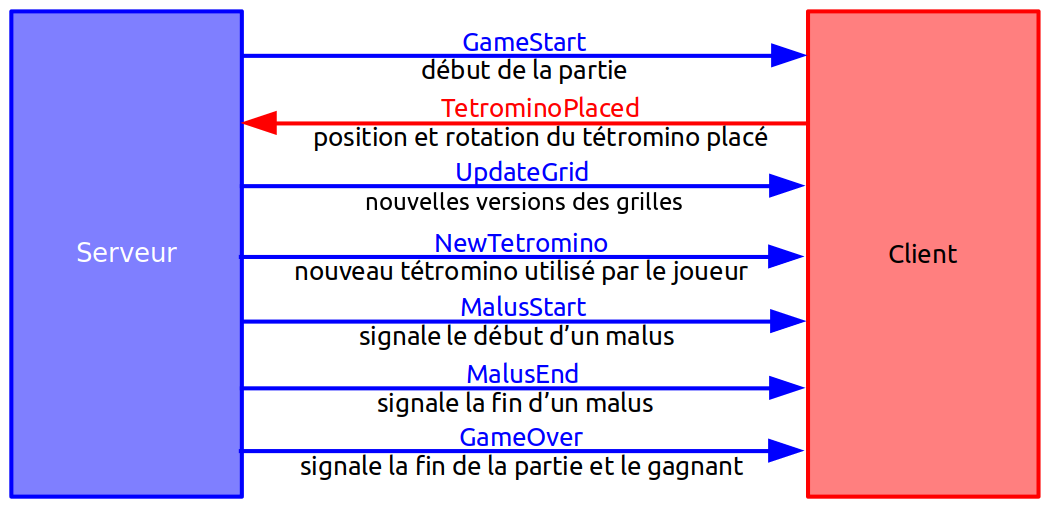
\includegraphics[scale=0.35]{img/ech.png}
				\caption{Représentation simplifiée des échanges de messages entre les clients et le serveur}
				\label{fig:echange}
			\end{figure}


			\subsubsection{Les messages du serveur vers le client}

				\paragraph{\texttt{Game\_start}} : message de début de partie, signale le début de la partie aux clients lorsque les deux joueurs sont prêts à jouer. Contient : 
					\begin{itemize}
						\item un tétromino qui sera mis en jeu par le clients
						\item un tétromino de prédication qui sera le prochain joué par le client
						\item la durée de la partie
					\end{itemize}

				\paragraph{\texttt{Game\_over}} : message de fin de partie, il indique au joueur s'il a gagné, perdu ou s'il y a une égalité. Contient :
					\begin{itemize}
						\item les scores des deux joueurs
						\item si la partie est gagnée, perdue ou s'il y a égalité
					\end{itemize}

				\paragraph{\texttt{New\_tetromino}} : message contenant le prochaine tétromino qui sera utilisé par le client. Contient :
					\begin{itemize}
						\item prochain tétromino utilisé par le client
					\end{itemize}

				\paragraph{\texttt{Update\_Grid}} : message qui contient la grille de jeu du joueur. Contient :
					\begin{itemize}
						\item la grille de jeu du joueur qui remplacera la précédente contenue dans le client
						\item le score
					\end{itemize}

				\paragraph{\texttt{Update\_Other\_Grid}} : message qui contient la grille de l'adversaire, pour l'afficher. Contient :
					\begin{itemize}
						\item la grille de jeu de l'adversaire, qui sera affiché à la place de l'ancienne
						\item le score de l'adversaire
					\end{itemize}

				\paragraph{\texttt{Malus\_start}} : signale le début d'une période malus pour le joueur ainsi que le type du malus qui s'applique. Contient :
					\begin{itemize}
						\item type du malus, indiquant ses effets
						\item la cible, indiquant si le client doit appliquer les effets ou s'il doit simplement indiquer que son adversaire est sous l'effet d'un malus
					\end{itemize}

				\paragraph{\texttt{Malus\_End}} : signale la fin de la période de malus actuelle. Contient : 
					\begin{itemize}
						\item la cible, indiquant si le client doit arreter d'appliquer les effets, ou si il doit arreter l'affichage du malus adverse
					\end{itemize}

			\subsubsection{Les messages du client vers le serveur}

				\paragraph{\texttt{Tetromino\_placed}} : contient le tétromino avec sa position et son orientation tel qu'il viens d'être placé par le joueur. Contient :
					\begin{itemize}
						\item un tétromino qui vient d'être placé par le joueur
					\end{itemize}
				\paragraph{\texttt{Connection\_lost}} : message signalant une déconnexion du joueur. Contient :
					\begin{itemize}
						\item la raison de la déconnexion
					\end{itemize}
			

\section{La communication}
	\subsection{Le serveur}

		Le serveur est la clé de voute du jeu. Il fait le lien entre les deux clients et gère l'évolutions du jeu.

		\subsubsection{La structure du serveur}

		Selon notre paradigme, le server fait loi, par conséquent, il contient toutes les informations nécéssaires pour le déroulement de la partie. Ainsi, pour chaque client, il contient : 
			\begin{itemize}
				\item une socket qui permet de communiquer avec le client
				\item une file contenant les messages de la part du client attendant d'être traité
				\item la grille de jeu du client, avec toutes les cases du jeu
				\item son score
				\item un vérificateur de triche
				\item un gestionnaire de malus, définissant quel malus est en cours pour le client et le temps restant pour le malus
			\end{itemize}

		Le serveur doit écouter les messages de la part des deux clients. Cependant, l'éxecution du serveur ne peut être interomput en attendant la reception d'un message. Nous avons donc créé deux threads d'écoute, chacun écoutant une socket associée à un client. 

		Lorsqu'un message est réceptionné, il est stocké dans la file du client en question. La file est partagée entre le thread d'écoute et le thread principal. \'A chaque tour de boucle, le thread principal regarde s'il y a un message stocké dans le file. Si c'est le cas, il traite ce dernier, met à jour les données du client et renvoit des message aux clients si besoin est.

		La figure \ref{fig:ser} représente la structure du serveur avec ses différents threads, ainsi que les files et les sockets des clients qui sont partagées par ces derniers.

		\begin{figure}[bt]
			\centering
			\includegraphics[scale=0.3]{img/ser.png}
			\caption{Représentation simplifiée de la structure du serveur}
			\label{fig:ser}
		\end{figure}

		\subsubsection{Le traitement des messages}
			Le serveur peut recevoir deux messages de la part du client : \texttt{Connection\_Lost} et \texttt{Tetromino\_placed}.

			Le message \texttt{Connection\_Lost} sert à indiquer que le client se déconnecte du serveur, la partie est donc terminée et permet au serveur et au client de se fermer correctement. Dans ce cas, le serveur envoit un message \texttt{Game\_over} à l'autre client --- le désignant comme le vainqueur --- et arrête son exécution.

 
			Le message le plus fréquent sera \texttt{Tetromino\_Placed}. Sa réception indique que le joueur viens de placer le tétromino avec lequel il jouait. Ce message contient le type de tétromino, sa position et sa rotation. 

			D'abord le serveur vas commencer par vérifier qu'il n'y a pas eu de triche --- ce procédé sera décrit en détail dans la partie suivante. 


			La grille du joueur correspondant est ensuite mise à jour avec le tétromino reçu.
			Si une ligne est complétée, elle est supprimée, ce qui augmente le score du joueur en question.


			Le malus est ensuite déterminé en fonction du nombre de ligne détruite :

			Si une ligne est détruite, aucun malus n'est envoyé.

			Si le joueur détruit deux lignes, le serveur envoi à chacun des joueurs un message \texttt{Send\_Malus\_Start}, avec le type de malus "rotation".

			\begin{itemize}
				\item le joueur reçoit un message indiquant que l'adversaire est le cible du malus
				\item l'adversaire reçoit un message indiquant qu'il est la cible du dit malus
			\end{itemize}

			Le cas est similaire si trois lignes détruites, avec simplement le type du message, qui sera "accéleration".

			Dans ces deux cas, une horloge se lancera au moment de l'envoi du message. Au bout de 10 seconde, un message \texttt{Send\_Malus\_End} sera envoyé de manière similaire aux deux clients.

			Si le joueur a effectué un tétris --- quatres lignes détruites --- un tétromino de type aléatoire est généré et placé aléatoirement en bas de grille de l'autre joueur. Les cases qui correspondent à ce tétromino seront supprimé de la grille l'empéchant de compléter des lignes.

			Après la gestion des malus, les deux grilles mises à jour seront envoyées aux deux clients.
				
		\subsubsection{Le système anti-triche}
			Comme nous l'avons vu, le serveur fait loi, nous avons donc décidé d'ajouter un système anti-triche au serveur.

			Le but est de vérifier que les données envoyé par les clients dans le message tétromino placed sont cohérente. 

			Pour ce faire, le serveur vas vérifier le temps entre les deux messages du client, donc le temps que le client a pris pour jouer un tétromino.

			A partir de la position du tétromino qui vient d'être placé, on calcul le temps maximum que celui-ci peut prendre pour arrivé à cet endroit. Donc sa hauteur multiplié par le temps de chute normal.
			S'il dépasse le mouvement est concidéré comme suspicieux.
			La vérification inclue aussi les potentiels malus en cours --- délai plus court en cas de malus d'accélération et vérification sur la rotation pour le malus rotation.

			Bien entendu si le réseau connais des problèmes lors du transfert du message, cela peu retarder l'arriver du messafe et donc fausser le calcul. Nous avons pris deux précaution contre cela. 

			D'abord nous avons ajouté une marge d'erreur de quelque seconde qui tiens compte de cette éventualité. Nous avons également prévu un système de fautes.

			Un délai trop long entre deux messages --- ou une rotation en cas de malus --- cause une faute, au bout de trois fautes, le joueur est concidéré comme un tricheur et est éliminé. Son adversaire est alors déclaré vainqueur.


			Ce système anti-triche peut être amélioré, notament en vérifiant que la position du tétromino est bien atteignable depuis le haut du tableau.

			Le serveur est donc la plaque tournante des communications du jeu, gérant et contrôlant les messages qu'il échange avec les clients. 

	\subsection{La sérialisation}

		Les échanges des messages vus précédemment nécessite une sérialisation afin qu'ils puissent être envoyés par les sockets, ces dernières ne pouvant envoyés que des tableaux d'octet.

		Pour ce projet, nous avons réalisé notre propre bibliothèque de sérialisation. Nous nous sommes inspirés des bibliothèques de sérialisation de GamedevFramework ainsi que de SFML/Packet. 
		Notre sérialisation est organisée en deux classe symétrique : Serializer et Deserializer, qui sont communes au serveur et aux clients. Elles contiennent tous les deux un tableau dynamique d'octet qui représente les informations sérialisés ainsi qu'une position d'écriture ou de lecture, respectivement pour le sérialiseur et le désérialiseur. 
		
		\subsubsection{Sérialisation des types simples}

		Pour la sérialisation des type simple nous utilisons une méthode templatée privée qui peut sérialiser n'importe quel type simple. Cette sérialisation est ensuite appelé par d'autre méthode auxquelles sont assignés des types spécifiques afin d'éviter la sérialisation de type non-désiré.
		
		L'endianess de cette méthode de sérialisation, c'est-à-dire l'ordre séquentiel dans lequel sont ranger nos données sérialisées, définit l'endianess de toute notre sérialisation. Celle-ci est au format Big-Endian pusique celui-ci est le format par défaut des infrastructures réseaux. Cela signifie que l'octet le plus significatif (octet de poid fort) est stocker en premier dans notre sérialisation et est donc envoyé en premier lors des échanges. Par exemple dans la figure \ref{fig:serial}, l'octet de valeur 0xAA est placé avant l'octet de valeur 0xBB dans le tableau d'octet lors de la sérialisation.

		\begin{figure}[bt]
			\centering
			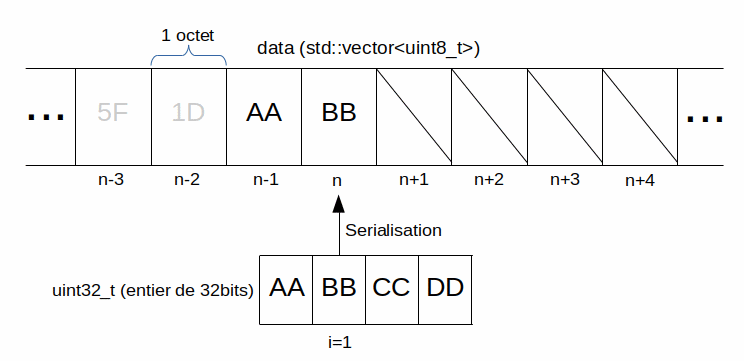
\includegraphics[scale=0.35]{img/serialisation.png}
			\caption{Représentation simplifiée de la sérialisation d'un entier de 32bit, est ici représenté la sérialisation du second octet avec la position d'écriture égale à n.}
			\label{fig:serial}
		\end{figure}

		\subsubsection{La sérialisation des types complexes}

		L'objectif étant de pouvoir sérialiser des messages, il nous faut pouvoir sérialiser des types complexes : objets ou structures. Pour cela nous sérialisons chaque attributs du type complexe que l'on souhaite échanger. Si l'attribut est un type simple alors on utilise la sérialisation des types simples vu précédemment sinon on fait appel la sérialisation du type complexe correspondant à l'attribut, cela jusqu'à la sérialisation complète de notre type complexe.

		\subsubsection{La sérialisation des messages}

		Nos messages sont répartis en deux structures, une pour les échanges client vers serveur et une pour les échanges serveur vers client. Chacune de ces structures contient une union contenant les structures des messages ainsi que le type du message représenté par une énumération : c'est une union taguée.

		Les structures de messages contiennent ensuite ce que chaque message doit envoyer, des types simples ou des types complexes. 
		
		La sérialisation des messages est donc la suivante : on sérialise tout d'abord le type de message puis la structure de message présente dans l'union correspondante au type du message.

		\subsubsection{La déserialisation}

		Comme précédemment évoquer, le Deserializer est le symétrique du Serializer, de ce fait la déserialisation va effectuer les opérations inverse de la sérialisation. Pour le cas des messages, le Deserializer va d'abord déserialiser la type du message pour savoir quelle méthode appeler pour deserialiser le reste du message.

		\subsubsection{Une seule asymétrie entre Serializer et Deserializer}

		Une seule asymétrie entre Serializer et Deserializer existe, il s'agit de la gestion de la taille du message. Car pour envoyé notre message sur une socket, nous devons connaitre sa taille et la spécifier. Pour cela le sérialiseur garde toujours huit octets en début de son tableau dynamique pour que lorsqu'on récupère le tableau d'octet, la taille du tableau soit insérée au debut de celui-ci. Ainsi cela permet lors de la réception du message, de lire les huit premiers octets pour connaitre la taille du message et alloué un tableau dynamique de la bonne taille pour enfin l'assigner à un déserialiseur.

	
	\section{La jouabilité}
		\subsection{Les structures de données communes}

		\subsubsection{Tetromino}

			Le tirage au sort de tétromino se fait du coté serveur. Le serveur envoie ensuite les données concernant les tétrominos aux clients.
			
			Au début de la partie, le client récupère les données du premier tétromino en jeu, \texttt{currentTetro} et les données du tétromino suivant, appelé \texttt{nextTetro} grâce au message GameStart.
			Pour la suite de la partie, lorsque le tétromino en jeu se pose, le client le signal au serveur, avec le message \texttt{Tetromino\_Placed}. Le serveur renvoie le message \texttt{New\_Tetromino} au client contenant les données d’un nouveau tétromino. Ce nouveau tétromino prend la place du tétromino de prédiction ( \texttt{nextTetro}) alors que l’ancien \texttt{nextTetro} devient le \texttt{currentTetro} et entre en jeu.

			La classe Tétromino contient les informations sur un tetromino :
			\begin{itemize}
				\item son type
				\item son sens de rotation actuel
				\item sa forme représenté pas une matrice de 4x2
				\item la position de son ancre représenté par un vecteur (x, y)
			\end{itemize}

			\paragraph{ \texttt{getCases()}} :
			cette fonction permet de récupéré la liste des coordonnées des cases du tétromino.
			\begin{enumerate}

				\item On récupère les coordonnées de l’ancre ainsi que sa place dans la matrice 2x4 représentant la forme du tétromino
				\item On récupère l’entier représentant la rotation du tétromino
				\item Suivant la rotation du tétromino, le sens du parcours de la matrice 2x4 est différent
				\item Si on est sur une case contenant une partie du tétromino soit une case avec un entier différent de 0, on ajoute les coordonnées de cette case, sous forme de vecteur, dans la liste à retourner
				\item Une fois le parcours de la matrice terminé on renvoie la liste de coordonnées

			\end{enumerate}



		\subsubsection{Grid}
			Pour représenter la zone de jeu nous utilisons un tableau d’entier à une dimension. Une case vide est représenté par un 0. 
			On crée le tableau avec l’objet \texttt{Grid}.

			\paragraph{Vérification des déplacements}
				La fonction Grid::movePossible permet de vérifier si l’action de déplacement faite par le joueur et valide. Elle prend en paramètre le Tétromino en jeu (tetromino qui chute et qui est contrôlé par le joueur) et un vecteur (x, y) pour savoir dans quel direction le mouvement est fait.

				Cette fonction est appelé dans : 
				\begin{itemize}
					\item \texttt{Grid::downPossible}, avec le vecteur {0, 1}
					\item \texttt{Grid::rightPossible}, avec le vecteur {1, 0}
					\item \texttt{Grid::leftPossible}, avec le vecteur {-1, 0}
				\end{itemize}

				La fonction \texttt{Grid::rotatePossible} permet d’autorisé où non la rotation de la pièce en jeu. La rotation peut être par exemple refusé si le tetromino est bloqué entre 2 autres tétrominos ou si il est sur le bord de la zone de jeu. Dans ces 2 cas, la rotation du tétromino le ferait soit passé a travers d’autre pièce ce qui est impossible ou encore sortir de la zone de jeu. On vérifie donc si les cases du tétromino après rotation sont bien dans la zone de jeu et qu'il n'y ai pas déjà un tétromino sur cette case grâce à la fonction \texttt{Tetromino::getCases}.

			\paragraph{Placement d’un tetromino}
				Si la fonction \texttt{Grid::downPossible} renvoie \texttt{false}, le tetromino actuellement en jeu est placé. Hors, seul son ancre est visible dans le tableau lors de sa chute, il faut donc ajouter toute les cases qui compose le tetromino dans la zone de jeu afin d’envoyé un nouveau tetromino en jeu.
				On appelle les fonctions \texttt{Tetromino::getCases} et \texttt{Tetromino::getType} pour placer toutes les cases du tétromino dans le tableau.

			\paragraph{Suppression de lignes}
				La fonction \texttt{Grid::deleteLines} parcours le tableau et détecte si des lignes sont pleine, elle est appelée lorsqu'un tétromino est posé.
				Si c’est le cas, elle appel la fonction \texttt{Grid::fallLines} sur la lignes correspondante.
				Elle renvoie le nombre total de ligne pleine qui ont été supprimé pour effectué le calcul du score et l’envoie de malus à l’adversaire.

				La fonction \texttt{Grid::fallLines} récupère en paramètre la ligne pleine, et fait descendre toutes les lignes au dessus de celle-ci d’une case vers le bas en commençant par le bas du tableau.

			\paragraph{Vérification de l’état de la grille}

				La fonction \texttt{Grid::gameOver} est appelé à chaque tétromino posé. Elle vérifie si les lignes du haut du tableau sont vide. Si une pièce est présente dans cette zone, on estime que la zone de jeu est complètement remplis et que l’arrive d’un prochain tétromino est impossible, dans ce cas elle renvoie \texttt{true}. Et le tableau est vidé entièrement.

	\subsection{Le client graphique}

		Le client est la partie visible de l’application pour les joueurs. Son rôle est de recevoir les messages envoyé par le serveur, de capter les interaction du joueur sur la partie et de les transmettre au server et d’afficher les différents éléments composant la fenêtre de jeu.

		\subsubsection{Les structures de données}

			\begin{figure}[bt]
				\centering
				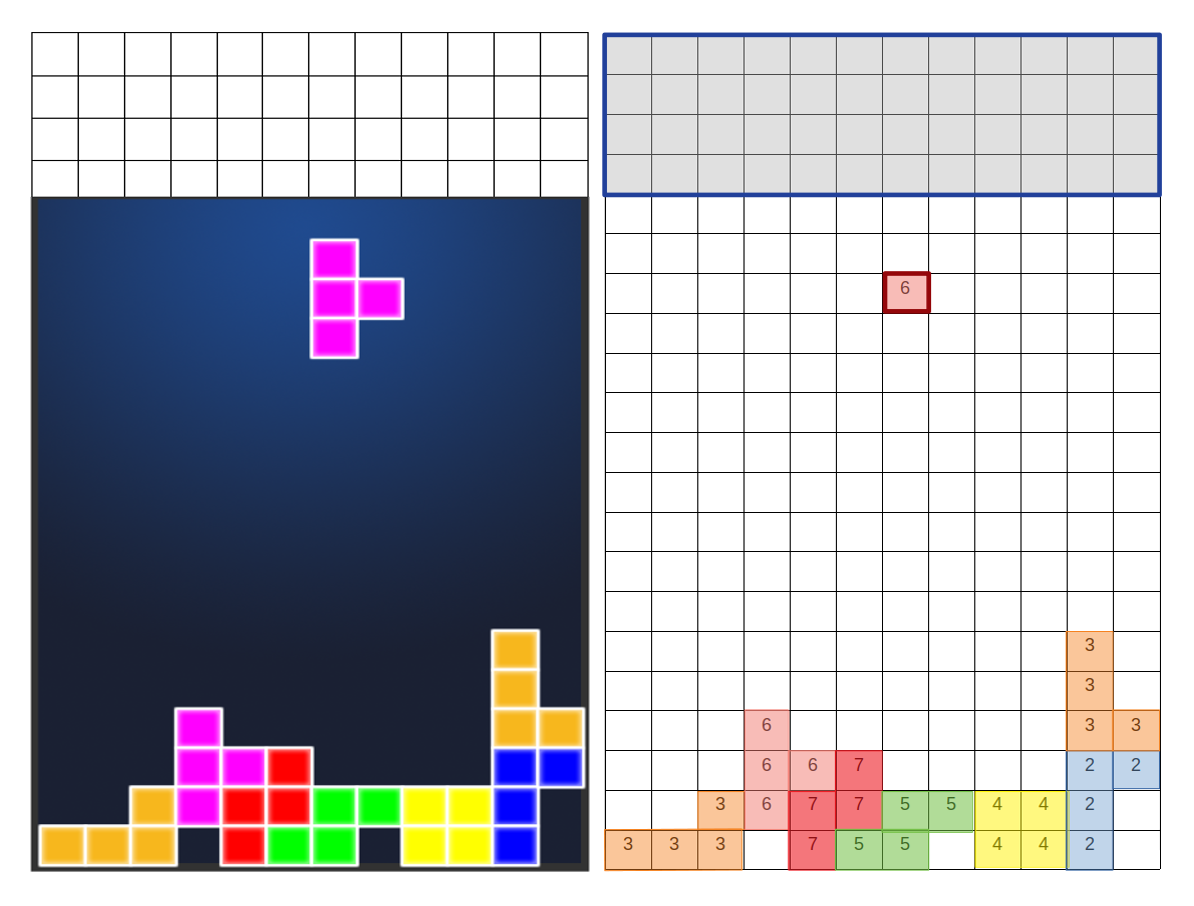
\includegraphics[scale=0.35]{img/grid.png}
				\caption{Représentation numérique des données dans le tableau de jeu}
				\label{fig:grid}
			\end{figure}

			\paragraph{Le tableau de la zone de jeu}

			Comme expliqué précédemment, notre zone de jeu est représenté par un tableau crée avec l’objet \texttt{Grid} de largeur 12 et de hauteur 21. Dans la figure \ref{fig:grid} nous avons représenté de façon schématique les données stockés dans ce tableau à un instant T d’une partie.

			Toute les case sans chiffres sont des cases contenant un 0. Nous voyons que le numéro stocké correspond au type du tetromino.

			Encadré en rouge nous avons l’ancre du tetromino actuellement en chute. Ce n’est qu ‘au moment de l’affichage que toute les case du tetromino sont récupéré. Pour la gestion de la chute, il nous etait plus simple de n’avoir qu’une seul case à déplacer. 

			Tout en haut du tableau de la zone de jeu, encadré en bleu, nous retrouvons 4 lignes qui n’apparaissent pas dans l’affichage pour le joueur.

			C’est 4 lignes nous permettent de faire apparaître le nouveau tetromino depuis le dessus de la zone de jeu et ce sont sur ces lignes que s’effectue le test \texttt{Grid::gameOver} pour savoir si la zone de jeu est entièrement remplie.


			\paragraph{GameArea}

			La classe GameArea est uniquement utilisé par le client. Elle contient tout les chargements des textures pour les sprites des différentes pièces.

			Nous avons un tableau de Sprite de largeur 12 et de hauteur 17 (on ne retrouve pas ici les 4 lignes du haut du tableau de la zone de jeu puisqu’elles ne sont pas affichée.

			On récupère les données stocké dans le tableau de la zone de jeu (\texttt{Grid}) à partie de la 5ème lignes et on modifie les sprite contenue dans le tableau de \texttt{gameArea}.

			La fonction \texttt{GameArea::setScale} utilise la classe \texttt{gf::Transformable} afin de modifié la taille de l’affichage en fonction de vecteur et ainsi nous permettre d’utilisé les même sprite pour la zone de jeu du joueur et celle du joueur adverse.

			\paragraph{Initialisation de la partie}

				Au tout début de la partie nous initialisons certains paramètre.

				Les score des 2 joueurs sont à 0
				Toute les cases des grilles de zone de jeu des 2 joueurs sont initialisés à 0
				Le booléen « enPartie » de notre boucle de jeu est passé a \texttt{true}
				Le client reçois le premier tetromino en jeu et le prochain tetromino
				Le timer est initialisé avec la duré de la partie


			\paragraph{Boucle de jeu}

			Notre boucle de jeu se repose sur le booléen \texttt{enPartie}

			Il passe à \texttt{false} si un des joueur quitte la partie ou le timer tombe à zero.

			Pendant la boucle de jeu le client:

	\begin{itemize}
		\item Recois les messages du server
		\item Récupère les actions du joueur
		\item Vérifie que les action faites par le joueur sont réalisable et mets a jour la position et la rotation du tetromino en jeu
		\item Si le tetromino est posé alors le tétromino de prédiction devient de le tétromino en jeu et il est placé en au de la grille de jeu, et le client envoie un message au serveur pour demander le prochain tetromino
	\end{itemize}

		Une fois toute les donnée mises a jour, l’affichage est réalisé et la boucle suivant commence

		Si le message concernant les malus est reçu alors certaine des données sont modifié jusqu’à ce que le temps de ce malus soit terminée.

		Si le booléen \texttt{enPartie} passe a \texttt{false} alors on sort de la boucle de jeu et on entre dans une autre boucle qui permet l’affichage final pour indiqué si le joueur à gagné ou perdu.

		A la réception des message du serveur :

		\texttt{Game\_Start} : 
		    Récupère et stocke les données du tétromino en jeu et du prochain tétromino.

		\texttt{New\_Tetromino} :
		    Récupère et stocke les données du prochain tétromino

		\texttt{Update\_Grid} : 
		    Mets à joueur l’affichage de la zone de jeu et du score du joueur

		\texttt{Update\_Grid\_Other} :
		    Mets à joueur l’affichage de la zone de jeu et du score du joueur adverse

		\texttt{Malus\_Start} : 
		    Vérifie sur quel joueur le malus s’applique.
		    Si c’est le joueur qui reçois un malus, on récupère le type du malus. On affiche le logo correspondant et la grille du joueur devient rouge.
		    Si c’est le joueur adverse qui reçois un malus, on affiche sa grille en rouge.

		\texttt{Malus\_End} :
		    Vérifie sur quel joueur le malus correspondant s’appliquait.
		    Si c’est le joueur qui est concerné alors on enlève le logo du malus de l’affichage et sa zone de jeu revient à la couleur initiale.
		    Si c’est le joueur adverse qui est concerné, on affiche sa zone de jeu de la couleur initiale.

		\texttt{Game\_Over} :
		    On récupère les résultats de la partie et on passe le booléen de la boucle de jeu à \texttt{false}.

		\texttt{Connection\_Lost} : 
		    On passe le booléen de la boucle de jeu à \texttt{false}
		    

		\subsubsection{La fenêtre graphiques}

			\begin{figure}[bt]
				\centering
				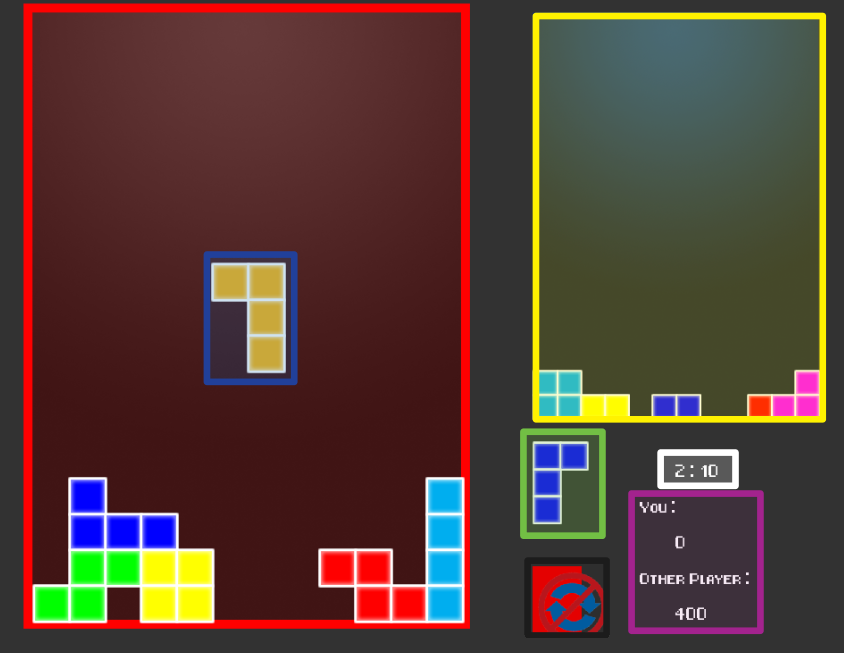
\includegraphics[scale=0.35]{img/fenetre.png}
				\caption{Différentes zone d'affichage de la fenêtre du jeu}
				\label{fig:fen}
			\end{figure}

			Les différents element composant notre ecran de jeu, tel qu'on peut les voir sur la figure \ref{fig:fen} : 

			En rouge : Zone du jeu du joueur. On y trouve les tetromino déjà posé ainsi que le tetromino en jeu en train de chuté. C’est avec cette fenetre que le joueur va intéragir.

			En jaune : Zone du joueur de l’adversaire. On ne vois pas la piece en jeu mais on voit les piece déjà posé. Le joueur peut alors voir si son adversaire est en difficulté ou si au contraire une ligne est sur le point d’etre formée.


			Ces 2 zones sont crée grace au classe \texttt{Grid}, et \texttt{Game Area} ainsi qu’en utilisant la classe \texttt{gf::Transformable}.

			En vert : Prochaine pièce

			En blanc : le timer

			En violet : Les scores des 2 joueurs

			En noir : Affichage du malus en cours. Si aucun malus n’est actif cette partie de l’écran est vide. Une jauge de couleur rouge permet de savoir approximativement le temps qu’il reste pour que le malus se termine


		\subsubsection{Les actions du joueur}

			Lors de la chute du tetromino en jeu, le joueur peu intéragir sur celui ci avec les touche du clavier :

			Les flèches gauche et droite permettent de déplacer latéralement le tétromino.
			La flèche du bas permet d’accélérer la chute si on reste appuyé dessus.
			La barre d’espace permet de faire tourné le tetromino sur lui même.

			De plus, la fermeture de la fenêtre étant aussi une action du joueur sur le jeu, elle fait partie de la liste des contrôle.


			Pour capter les actiosn réalisés par le joueur nous avons crée une classe \texttt{Controls}.

			Dans cette classe nous définissons des objets de classe \texttt{gf::Action}.

			Pour les actions lié à une touche de clavier nous utilisons la fonction \texttt{gf::Action::addScancodeKeyControl} avec le \texttt{gf::Scancode} correspondant à la touche voulue.

			Nous avons aussi une fonction \texttt{reset} qui permet de stoppé toute les actions en cours. Nous l’utilisons dans la boucle de jeu.
	
	

\section*{Conclusion}

Le jeu que nous avons développé est fonctionnel et il remplit le cahier des charges fixé au début du projet. 
Nous avons trouvé le projet très intéressant et il nous a permis d’acquérir de multiples connaissances et compétences. 

Nous avons pu notamment découvrir les bibliothèque Gamedev Framework et Boost::asio. Nous n’avions que très peu de connaissances en C++ en commençant le projet, la prise en main de ces bibliothèques n’a donc pas était facile au début. De plus, le principe de sérialisation ainsi que les méthodes utilisées nous étaient inconnues.

Grâce à ce projet nous avons donc pu mettre en pratique les connaissances et compétences de certaines matières de licence 2 et licence 3 (Algorithme et Programmation, Système, Système et Réseaux, Théorie des langages, Programmation Multi-Paradigmes) mais aussi les améliorer.

Les objectifs principaux de notre projets ont été remplis, or des améliorations sont encore possibles.
Nous pourrions par exemple améliorer le système anti-triche ou encore créer un systèmes de personnalisation de partie permettant de jouer à plus de 2 joueurs.


\end{document}